\documentclass[12pt]{beamer}
%\documentclass[handout,xcolor=pdflatex,dvipsnames,table,12pt]{beamer}
\usepackage[latin1]{inputenc}
%\usepackage[T1]{fontenc}
\usepackage{amsmath} % for math AMS fonts
\usepackage{graphicx} % to include figures
\usepackage{subfigure} % to have figures in figures
\usepackage{multimedia} % to include movies
\usepackage{listings} % to display code
\usepackage{colortbl} % colored tables
\usepackage[latin1]{inputenc} % support for accented letters, etc.
\usepackage{amsthm}
\usepackage{hyperref}
\usepackage{ulem}

\usetheme{Warsaw}
\setbeamercovered{transparent}

\title[Introduction to Cryptography]{Hard Drive Encryption}
\author{Christian Mann -- christian-mann@utulsa.edu}
\institute{University of Tulsa\\
Tulsa, Oklahoma 74104}
\date{\today}

\logo{
\includegraphics[height=1.5cm]{pictures/SFSLogoMain}}

\begin{document}

\lstset{
language=python,                % choose the language of the code
%basicstyle=\footnotesize,       % the size of the fonts that are used for the code
%numbers=left,                   % where to put the line-numbers
%numberstyle=\footnotesize,      % the size of the fonts that are used for the line-numbers
%stepnumber=2,                   % the step between two line-numbers. If it's 1 each line will be numbered
%%umbersep=5pt,                  % how far the line-numbers are from the code
%backgroundcolor=\color{white},  % choose the background color. You must add \usepackage{color}
showspaces=false,               % show spaces adding particular underscores
showstringspaces=false,         % underline spaces within strings
showtabs=false,                 % show tabs within strings adding particular underscores
%%frame=single,	                % adds a frame around the code
tabsize=4,	                % sets default tabsize to 2 spaces
%%captionpos=b,                   % sets the caption-position to bottom
%%breaklines=true,                % sets automatic line breaking
%%breakatwhitespace=false,        % sets if automatic breaks should only happen at whitespace
%%title=\lstname,                 % show the filename of files included with \lstinputlisting; also try caption instead of title
%escapeinside={\%*}{*)}          % if you want to add a comment within your code
%morekeywords={*,...}            % if you want to add more keywords to the set
}

\newtheorem{mydef}{Definition}


\begin{frame}
\titlepage
\end{frame}


% no outline

% note, you should have three sections maximum.  two is good.  subsubsections are evil.
% new slides begin with teh \begin{frame} and end with \end{frame}

\iffalse
Generic Block Cipher description
Block cipher functional description
Block cipher design
Block cipher modes, at least 4.
algorithms
weaknesses
how to break a block cipher
\fi

\begin{frame}{Hard Drive Encryption}{}
\begin{block}{Important Properties}
	\begin{itemize}
		\item Confidentiality
		\item Speed
		\item Disk Space Efficiency
	\end{itemize}
\end{block}
\end{frame}

\begin{frame}{Hard Drive Encryption}{Confidentiality}
\begin{block}{Adversary Tools}
\begin{itemize}
	\item Can read raw encrypted sectors at any time (COA)
	\item Can supply plaintext to be stored on disk, encrypted (CPA)
	\item Can modify unused sectors on disk and request decryption (CCA)
\end{itemize}
\end{block}

\begin{block}{Goal}
A method provides good confidentiality if the only information that an adversary
can determine over time is whether the data in a sector has or has not changed
since the last time they looked.
\end{block}
\end{frame}

\begin{frame}{Hard Drive Encryption}
	\centering
	We must process each sector differently, so that an attacker can't just copy one
	file into an unused sector and decrypt it.
\end{frame}

\begin{frame}{Hard Drive Encryption}{Encryption Type}
\begin{block}{Stream Ciphers}
	Each sector must be encrypted differently, so a stream cipher might work..
	but we need to store a nonce per sector, which is generally considered a
	waste of space. This nonce also needs to be updated every time the data
	changes
\end{block}
\begin{block}{Block Ciphers}
	Which mode of operation? \begin{description}
		\item[ECB] Clearly a bad choice -- penguins will be visible
		\item[CTR, OFB] Actually stream ciphers
		\item[CBC] Viable. Need to store an IV per sector.
	\end{description}
\end{block}
\end{frame}

\begin{frame}{Hard Drive Encryption}{Integrity?}
	\centering
	None! \textit{Most HDD encryption schemes provide no form of integrity
	verification}. Partially, this is because a replay attack is always
	possible. Partially, this just isn't what HDD encryption is concerned with.
	Use a MAC or something if you care.
\end{frame}

\begin{frame}{Cipher Block Chaining}{}
	\[ C_i = E_K(C_{i-1} \oplus P_K) \]

	This is applied per-sector, with a different (unpredictable!) IV in each sector.
\end{frame}

\begin{frame}{Cipher Block Chaining}{Watermark Attack}
	If the IVs for two sectors are related, an attacker can do a ``watermarking
	attack,'' a chosen plaintext attack:

	Construct a file that spans multiple sectors, with contents such that:
	\begin{align*}
		P_1 \oplus P_2 &= IV_1 \oplus IV_2 \\
		P_1 \oplus IV_1 &= P_2 \oplus IV_2 \\
		E_K(P_1 \oplus IV_1) &= E_K(P_2 \oplus IV_2) \\
		C_1 &= C_2
	\end{align*}

	\begin{alertblock}{}
		The attacker can detect that this file has been written to disk!
	\end{alertblock}
\end{frame}

\begin{frame}{Cipher Block Chaining}{ESSIV}
	Preventing predictable IVs -- we don't want to generate a random one because
	space restrictions. We can use a function of the sector number:
	\begin{align*}
		IV(n) &= E_s(n) \\
		s &= hash(K)
	\end{align*}
	\centering
	``Encrypted Salt-Sector Initialization Vector''

	\begin{itemize}
		\item Still does not prevent all the fun attacks from Lab 3
	\end{itemize}
\end{frame}

\begin{frame}{LRW}{Liskov, Rivest, Wagner; or, remember modern algebra?}
	Encrypts each block individually:
	\begin{align*}
		C &= E_K(P \oplus X) \oplus X \\
		X &= F \otimes I
	\end{align*}
	where $K$, $F$ are encryption keys; $I$ is the block's index.

	These operations are performed in $GF(2^{128})$, the AES field.
\end{frame}

\begin{frame}{LRW}{Overall Idea}
\begin{block}{Tweakable Encryption}
	Previously, we had $E(K, P)$.
	
	We now want $E(K, T, P)$ such that:\begin{enumerate}
		\item every value of $T$ still gives secure encryption, and
		\item going from $E(K, T, P)$ to $E(K, T', P')$ is easy.
	\end{enumerate}

	Influential paper: ``Tweakable Block Ciphers''. Liskov, Rivest, Wagner.
	2005.
\end{block}
\end{frame}

\begin{frame}{XEX}{XOR Encrypt XOR}
	Similar to LRW:
	\begin{align*}
		X &= E_K(I) \otimes \alpha^j \\
		C &= E_K(P \oplus X) \oplus X
	\end{align*}
	where $K$ is an encryption key;
	$I$ is sector number;
	$j$ is block number within sector;
	$\alpha = 2$, a generator in $GF(2^{128})$.

	This is good for sequential access -- to get the next block, just multiply
	$X$ by $\alpha$; no need to re-encrypt $I$.
\end{frame}

\begin{frame}{Ciphertext Stealing}{Alternative to padding}
	\centering
	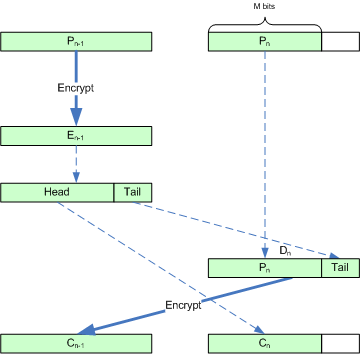
\includegraphics[width=\textwidth, height=0.8\textheight, keepaspectratio=true]{pictures/CTS_ECB_Encryption.png}
\end{frame}

\begin{frame}{XTS}{XEX-based Tweaked-codebook mode with Ciphertext Stealing}
	\centering
	\pgfimage[width=\textwidth]{pictures/XTS_encryption.svg.png}
\end{frame}

\begin{frame}{XTS}{Details}
	\begin{itemize}
		\item Uses two keys: someone misunderstood the spec \\
		\item Default in TrueCrypt, VeraCrypt, FileVault 2 \\
		\item Supported by every important software \\
		\item Can be considered the ``default.''
	\end{itemize}
	\begin{alertblock}{Integrity}
		XEX, LRW, XTS do not provide \textit{any} amount of integrity checking!
		The attacker (if possible) might replace 16-byte blocks at will,
		possibly with previous blocks of valid files (at that location)!
	\end{alertblock}
\end{frame}

\begin{frame}{Questions / Comments?}{}
\end{frame}

\end{document}
